\documentclass[tikz,border=5pt]{standalone}
\usepackage{amsmath}
\usetikzlibrary{arrows.meta,positioning,calc,fit,backgrounds}

\definecolor{siteaccent}{RGB}{54,117,138}
\definecolor{sitelight}{RGB}{238,245,247}
\definecolor{siteborder}{RGB}{190,211,218}
\definecolor{sitetext}{RGB}{32,39,43}
\definecolor{sitemuted}{RGB}{102,116,123}

\tikzset{
  block/.style={draw=siteborder, fill=sitelight, rounded corners=2pt,
    minimum width=23mm, minimum height=12mm, align=center, inner xsep=4pt, text=sitetext},
  strong/.style={draw=siteaccent, fill=white, rounded corners=2pt,
    minimum width=25mm, minimum height=12mm, align=center, inner xsep=4pt, text=sitetext},
  flow/.style={-{Latex[length=2.2mm]}, semithick, draw=siteaccent}
}

\begin{document}
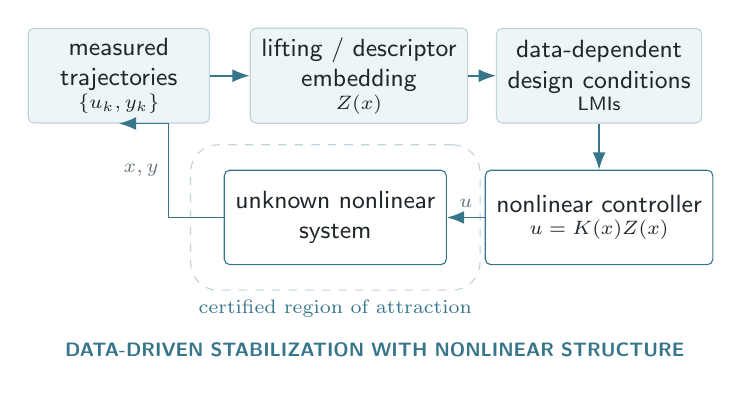
\begin{tikzpicture}[font=\sffamily\small]
  \node[block] (data) at (0,1.65) {measured\\trajectories\\[-1mm]\scriptsize $\{u_k,y_k\}$};
  \node[block] (embed) at (3.05,1.65) {lifting / descriptor\\embedding\\[-1mm]\scriptsize $Z(x)$};
  \node[block] (design) at (6.1,1.65) {data-dependent\\design conditions\\[-1mm]\scriptsize LMIs};
  \node[strong] (controller) at (6.1,-0.15) {nonlinear controller\\[-1mm]\scriptsize $u=K(x)Z(x)$};
  \node[strong, minimum width=27mm] (plant) at (2.75,-0.15) {unknown nonlinear\\system};

  \draw[flow] (data) -- (embed);
  \draw[flow] (embed) -- (design);
  \draw[flow] (design) -- (controller);
  \draw[flow] (controller) -- node[above, text=sitemuted, font=\scriptsize] {$u$} (plant);
  \draw[flow] (plant.west) -- ++(-0.7,0) |- node[pos=0.25, left, text=sitemuted, font=\scriptsize] {$x,y$} (data.south);

  \begin{scope}[on background layer]
    \node[draw=siteborder, dashed, rounded corners=10pt, fit=(plant),
      inner xsep=12pt, inner ysep=9pt, label={[text=siteaccent,font=\scriptsize]below:certified region of attraction}] {};
  \end{scope}

  \node[anchor=north, text=siteaccent, font=\sffamily\scriptsize\bfseries]
    at (3.25,-1.62) {DATA-DRIVEN STABILIZATION WITH NONLINEAR STRUCTURE};
\end{tikzpicture}
\end{document}
